% chap3.tex
%

\newif\ifcompress
\compresstrue   % Uncomment this line for the authors
\compressfalse % Uncomment these two lines for anonymous review

\mychapter{Structured and Unstructured Data for Factoid Question Answering}

\noindent

In this work I propose to enrich the input data representation for QA systems by combining available unstructured, semi-structured and structured data sources for joint reasoning, which can improve the performance of question answering over both text collections and knowledge bases.


\section{Improving Knowledge Base Question Answering using Unstructured Text Data}

\subsection{Relation extraction for Knowledge Base completion}

\subsubsection{Relation extraction from Question-Answer pairs}
This is my work from NAACL student research workshop.

\subsubsection{Question-guided relation extraction}
The idea is that we can aggregate related questions and relation extraction patterns.
When a person asks a question, we retrieve passages and sentences to extract the answer from.
Imaging a question is asking a certain property of an entity.
If we can retrieve a sentence, that mentions this entity along with a candidate answer, we can build a pattern for relation extraction.
This pattern will be connected to the question ``template''.
Likewise, if we already have relation extraction patterns we can boost those that are retrieve in response to the question and save this connection.

Hypothesis:
\begin{enumerate}
\item Patterns retrieved in response to the question are better in quality, we can boost them. We can try to verify this on some relation extraction dataset and questions from some query log. We can also try to use some KBQA dataset.
\item Patterns mined for questions should help question answering. This is essentially weak supervision for training knowledge base question answering using text based question answering.
\end{enumerate}

Problems:
\begin{itemize}
\item How to extract new predicates? If we have a question, and a sentence is mentioning a pair of non-related entities, how can we make a new one?
\item How to deal with more complex questions, that are not simple relations
\end{itemize}

Useful dataset: MSN query log, SimpleQuestions from Facebook, WebQuestions, NYT relation extraction dataset.

\subsection{Question Answering over Knowledge Bases with External Text Data}
This is Text2KB SIGIR submission.

\subsection{Answer ranking approach for Knowledge Base Question Answering}

\begin{enumerate}
\item Use entity search to retrieve a set of candidate answer entities
\item Predict which entity should be returned as the answer
    \begin{itemize}
    \item independently for each entity
    \item jointly - select a set of entities as the answer. This should be better, can account for the size and homogeneity of the answers
    \end{itemize}
\end{enumerate}

We can index textual data that mention entities to improve entity ranking? Can we just rank Wikipedia pages?

\section{Semantic Text Annotations for Hybrid Question Answering}

In my thesis I propose to annotate text document collection with links to mentioned knowledge base entities.
Such semantic annotations open up many opportunities for QA reasoning, because it allows one to go from the information stored in text to structured data and vice versa.

More specifically, I propose the following factoid QA system architecture:
\begin{itemize}
\setlength\itemsep{0em}
\item \textbf{Pre-processing}: identify mentions of KB entities in text document collection and index the documents text and mentions in separate fields
\item \textbf{Topical entity identification}: search the text collection using question (or reformulated question \cite{AgichteinLG01}) as a query and use an approach similar to \cite{cornolti2014smaph} to detect question topical entities
\item \textbf{Candidate generation from text}: extract candidate answer (or intermediate answer) entities with evidence from the retrieved text documents using existing techniques, e.g. \cite{tsai2015web}.
\item \textbf{Candidate generation from KB}: explore the KB neighborhood of question topical entities and entities extracted from text documents on the previous step
\item \textbf{Candidate generation from KB \& Text}: use entity and text index to find entities mentioned near question topical entity and question terms in the document collection
\item \textbf{KB evidence extraction}: match neighbourhood of answer entities (entity type and other entities) against the question to get additional evidence
\item \textbf{Text evidence extraction}: estimate the similarity between the collection text fragments mentionining question and answer entities and the question text
\item \textbf{Rank candidate}: rank candidate answers using evidence extracted from the KB as well as from text
\end{itemize}

For example, for the question mentioned in the introduction \textit{``What republican senators supported the nomination of Harriet Miers to the Supreme Court?''} and a candidate answer sentence \textit{``Minority Leader Harry Reid had already offered his open support for Miers.''}, such joint text-KB representation can look like Figure \ref{fig:kb2text}.
A QA system can discover that ``Harry Reid'' political affiliation is with the Democratic Party, and he cannot be referred to as ``republican senator''.
In other cases using a KB as an additional source of information may reveal specific connections between entities in the question and in the answer candidates.
For example, for another TREC QA 2007 question \textit{``For which newspaper does Krugman write?''} and retrieved candidate answer \textit{New York Times} a path between ``Paul Krugman'' and ``New York Times'' in the knowledge graph gives an evidence in support of the candidate.

\begin{figure*}
\centering
 \begin{subfigure}[t]{0.45\textwidth}
 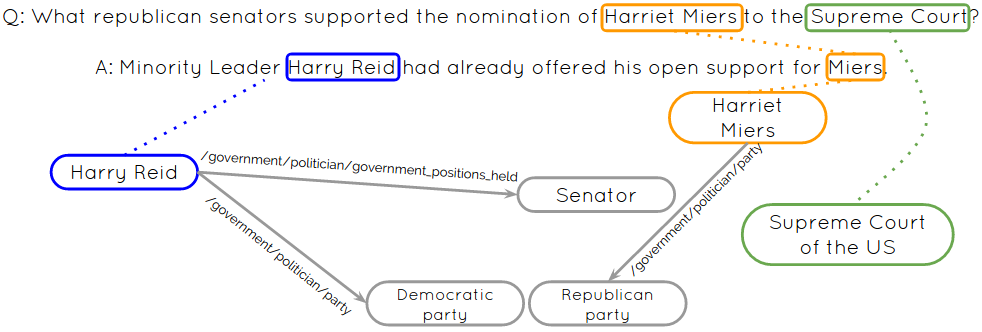
\includegraphics[width=\textwidth]{img/text_kb}
 \caption{Annotation of natural language text with mentioned entities and their subgraphs in a knowledge base}
 \label{fig:kb2text}
 \end{subfigure}
 \begin{subfigure}[t]{0.45\textwidth}
 \centering
 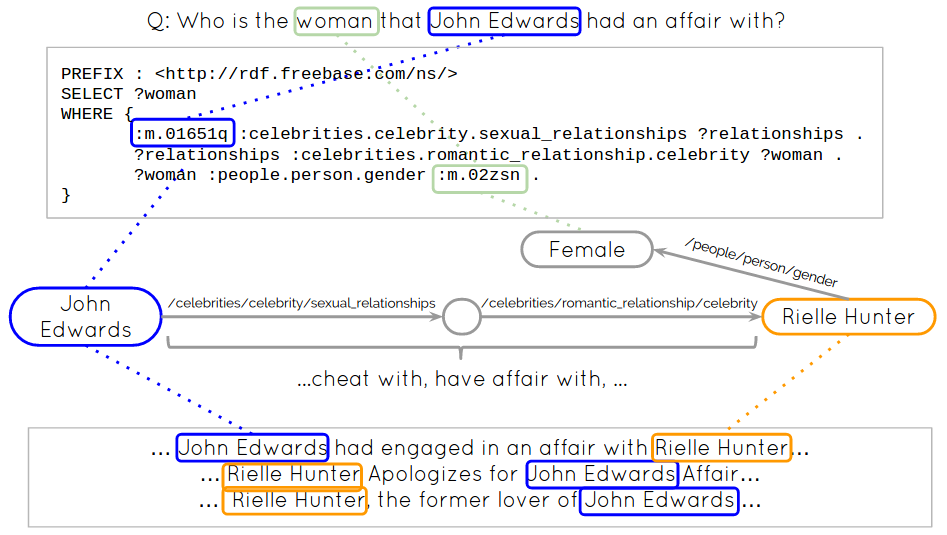
\includegraphics[width=\textwidth]{img/kb_text}
 \caption{Annotation of KB graph nodes and edges with unstructured text data}
  \label{fig:text2kb}
 \end{subfigure}
\label{fig:text_kb}
\vspace{-0.2cm}
\caption{Unstructured text and structured Knowledge Base connected via entity links for question answering}
\end{figure*}

Knowledge base question answering (KBQA) produce answers by constructing a structured query, that retrieves answer entities from the KB.
The main challenge in KBQA is mapping between natural language phrases in the question and knowledge base entities and predicates.
Such systems typically rely on the lexicon learned from the training data \cite{bastmore:cikm:2015:aquu,BerantCFL13:sempre,BerantL14:parasempre,yih:ACL:2015:STAGG,yao-scratch-qa-naacl2015}.
Such lexicons are often limited and needs to be retrained to include additional data.
The proposed approach allows a system to dig into the text resources that mention question and candidate answer pairs and use this information for scoring.
Figure \ref{fig:text2kb} shows a sample of data available for KBQA system to answer the \textit{`` Who is the woman that John Edwards had an affair with?''} question from a popular WebQuestions dataset \cite{BerantCFL13:sempre}.

\section{Evaluation}

\section{Experiments}

\subsection{Text-based QA}

TREC QA datasets served as a benchmark for various question answering systems.
Therefore, to evaluate the proposed approach for question answering over text enriched with the structured data I propose to test it on dataset derived from TREC QA and compare against existing strong baselines, including the most related approaches \cite{Fader:2014:OQA:2623330.2623677,Sun:2015:ODQ:2736277.2741651}.
The proposed system can use the web as the corpus and query it using Bing Search API\footnote{https://datamarket.azure.com/dataset/bing/searchweb}.
Freebase and Reverb extractions \cite{FaderSE11} are examples of schema-based and open knowledge bases that can be used for the experiments.
The metrics used for evaluation typically include accuracy and mean reciprocal rank (MRR).

For non-factoid question answering this year TREC pioneered a new question answering track - TREC LiveQA\footnote{http://trec-liveqa.org/}, which targets questions asked by real users of Yahoo! Answers website.
This year the deadline for system submission was on August 31 and my system trained on CQA QnA pairs participated in the challenge.
The results will be available on the TREC Conference in November 2015.
Organizers plan to continue with another TREC LiveQA task next year and this is going to be a good estimation of the effectiveness of the proposed techniques on hard real user questions.

\subsection{Knowledge base QA}

Most of the recent work on knowledge base question answering and semantic parsing have been evaluated on the WebQuestions dataset \cite{BerantCFL13:sempre}, which contains a collection of question text and correct answer entities.
The questions were collected using Google Suggest API and answers crowdsourced using Amazon Mechanical Turk\footnote{http://mturk.com/}
% Since the questions in the dataset come from Google search logs, it is a better approximation of real user needs and is cheaper to obtain than some previous benchmarks, e.g. Free917.
The proposed approach will be compared against the previous results\footnote{http://goo.gl/sePBja} on this dataset.
Again, web can be used as a text collection which can be queried using Bing Search API.
Relation extraction patterns can be mined using distant supervision from ClueWeb collection using publicly available dataset of Freebase annotations \cite{gabrilovich2013facc1}.

However, WebQuestions dataset has certain limitations, e.g. questions mined using Google Suggest API have very similar structure and lexicon, and to find the answer to the mined questions users were asked to use the question entity Freebase profile page,  which only include entities connected directly with a predicate or through a mediator node.
Therefore most of the state-of-the-art results on the dataset use a small number of predefined logical form patterns.
On the other hand CQA websites have a fraction of factoid questions with provided text answers.
Here I propose to use to construct a new dataset for question answering over Freebase by selecting a subset of QnA pairs with at least one entity in question and answer and some reasonable filtering heuristics and manual validation using crowdsourcing (e.g. through Amazon Mechanical Turk).
Existing systems need to be retrained and tested on the new dataset to compare against the proposed model.

% \subsection{Combined QA}
% To compare the proposed data enrichment approaches against the other available hybrid question answering systems I propose to use a dataset derived from TREC, such as the one used to evaluate the YodaQA system\footnote{https://github.com/brmson/dataset-factoid-curated}.
% The system combining unstructured and structured approaches to question answering can be run in parallel with results ranking using a machine learning model.

Datasets:
\begin{itemize}
\item TREC QA
\item WebQuestions
\item QALD
\item New dataset for factoid quetion answering derived from Yahoo! Answers data.
\end{itemize}

\section{Summary}


